\IEEEraisesectionheading{\section{Introduction}\label{sec:intro}}

\IEEEPARstart{L}{atent-factor} collaborative filtering is among the most accurate and widely deployed techniques in recommender systems, which select, from catalogues of millions of items, the few a user is likely to value \cite{gomez2016netflix,schafer2001ecommerce}. Matrix factorization represents each user and item by a short dense vector and predicts a rating as their inner product \cite{koren2009matrix,bennett2007netflix}. Alternating least squares (ALS) trains this model by solving, in every sweep, one regularized least-squares problem per user and per item \cite{zhou2008largescale}. Each problem requires a $K \times K$ Gram matrix and an $O(K^{3})$ solve for $K$ latent factors, so the cost grows quickly with the model size: a single run on the Netflix Prize data, with 80.6 million training ratings, performs about 31~TFLOP at $K=96$.

GPU implementations of ALS exist \cite{tan2016faster,gates2015accelerating,chen2021bals}, but nearly all compute in FP32 on conventional CUDA cores. NVIDIA's data-center and RTX GPUs since Volta also carry tensor cores, which execute a dense $16 \times 16 \times 16$ half-precision multiply--accumulate as a single warp-level operation \cite{markidis2018nvidia}. The RTX~3060 used here delivers about 25.5~TFLOP/s on tensor cores with FP16 inputs and FP32 accumulation, twice its 12.7~TFLOP/s FP32 peak, and data-center parts widen this ratio considerably. Deep learning exploits these units routinely \cite{micikevicius2018mixed}; explicit-feedback ALS does not, for three reasons. First, the rating matrix is highly sparse, so Gram assembly gathers scattered factor rows while tensor cores require dense operand tiles. Second, FP16 carries only 10 mantissa bits, and its effect on recommendation accuracy under the ALS normal equations has not been measured. Third, once the Gram stage is ten times faster, the batched Cholesky solves become the critical path.

This paper addresses all three obstacles with \textit{APR-BALS} (Adaptive-Precision Blocked ALS), a CUDA implementation of explicit-feedback ALS. Rating counts follow a long-tailed distribution, with ratings distributed highly unevenly across users and items, as shown in Fig.~\ref{fig:longtail}. Because rating counts are highly skewed, entities exhibit substantially different computational workloads; consequently, a single kernel configuration cannot provide efficient execution across all entities. APR-BALS therefore sorts users and items by rating count and dispatches them in three tiers: giant and dense entities assemble their Gram matrices on tensor cores, and the sparse tail runs on a register-tiled FP32 kernel. A custom blocked Cholesky solver keeps the solve stage from absorbing the gain\cite{gates2015accelerating}. The evaluation is built on an \textit{audited baseline}: the FP32 reference shares one binary, data layout, solver, and convergence rule with the accelerated path, so every reported ratio isolates the precision dispatch. The contributions of this paper are as follows.

\begin{figure}[!t]
\centering
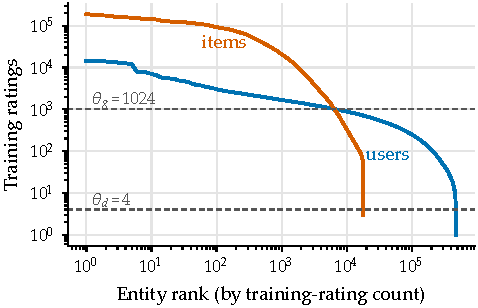
\includegraphics[width=\columnwidth]{figures/fig11_longtail.pdf}
\caption{Training ratings per user and per item in the Netflix Prize data, sorted by count. The dashed lines mark the giant and dense tier thresholds of Section~\ref{ssec:dispatch}.}
\label{fig:longtail}
\end{figure}

\begin{itemize}
\item \textbf{Density-adaptive tensor-core dispatch.} A three-tier dispatch sends more than $99.7\%$ of the training ratings to warp-level NVIDIA's Warp Matrix Multiply and Accumulate (WMMA) kernels that assemble only the upper triangle of each Gram matrix from gathered FP16 rows, with register prefetching and a multi-warp variant for very high-degree entities.
\item \textbf{A blocked batched Cholesky solver.} A $16 \times 16$-tile right-looking factorization with a fused forward solve and overlapped panel factorization runs $1.86$--$2.26\times$ faster than a tuned packed solver.
\item \textbf{An audited-baseline methodology.} A register-spill defect that crippled the FP32 baseline at $K \ge 48$, and would have inflated the speedups to $30$--$44\times$, was diagnosed and removed; no reported result uses the defective kernel. The same pitfall can affect any register-blocked Gram kernel whose accumulator footprint grows with $K^{2}$.
\item \textbf{Mechanism attribution.} A three-way ablation within one binary (FP16 WMMA, TF32 WMMA, and scalar FP32) attributes $87.8$--$99.6\%$ of the gain to the WMMA kernel at full FP32 range; reduced precision never contributes more than $1.32\times$.
\item \textbf{Comprehensive evaluation.} Speedups over the baseline reach $14.8\times$ on Netflix on an RTX~3060 and $10.8\times$ on a Tesla~T4, with test-RMSE changes below $0.005\%$ ($0.007\%$ on the T4) and run-to-run timing variation of at most $0.44\%$ over 100 runs. On identical data splits, APR-BALS is $3.0$--$6.4\times$ faster per iteration than NVIDIA's GPU-accelerated implementation of Collaborative Filtering using Alternating Least Squares (\textit{cuMF\_als})\cite{tan2016faster} and $3.4$--$4.1\times$ faster than a GPU-accelerated implementation of Collaborative Filtering using Coordinate Descent (\textit{cuMF\_CCD})\cite{yu2012scalable,nisa2017parallel}. Weighted regularization, solver-pipeline fusion, and heavy-ball momentum raise the end-to-end advantage over the baseline to $26\times$ ($19.5\times$ when iteration counts are matched.).
\end{itemize}

The evaluation covers NVIDIA Ampere and Turing GPUs and the latent dimensions $K \in \{16, 32, 48, 64, 96\}$ imposed by the WMMA tile shape; speedups on architectures with different FP16-to-FP32 throughput ratios are not established here. Section~\ref{sec:related} reviews related work, Section~\ref{sec:method} presents APR-BALS, Section~\ref{sec:eval} evaluates it against the FP32 baseline, Section~\ref{sec:extended} adds the shipped optimizations, Section~\ref{sec:external} compares it with external systems and discusses threats to validity, and Section~\ref{sec:conclusion} concludes.
